\chapter{Algorithm Description}

The algorithm described in this chapter and its preliminary test
result on real flight data was published in
\cite{zhang_obstacle_2012}. The program was implemented in Python
programming language \cite{_python_????}. An open source machine
vision library OpenCV was utilized to perform feature extraction and
tracking. The feature extraction method used was the Shi-Tomasi corner
detector \cite{shi_good_1994}. Feature tracking was accomplished
through the pyramid implementation of Lucas-Kanade optical flow method
\cite{bouguet_pyramidal_1999}. Both algorithms were implemented in
OpenCV. 

\section{Camera Centric Inverse Depth Parameterization}
The inverse depth parametrization by Civera \cite{civera_inverse_2008}
and camera centric coordinate system was adopted in this work with
some modification to integrate the inertial measurements. Figure
\ref{fig:algo1} shows the parameters definition in inverse depth
parameterization.

\begin{figure}[h]
\centering
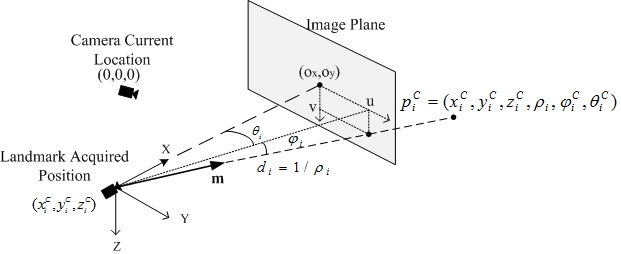
\includegraphics[width=10cm, keepaspectratio=true]{./Figures/idp.jpg}
\caption{Inverse Depth Parameterization}
\label{fig:algo1}
\end{figure}

A 3D scene point $p_{i}^{C}$ can be defined by 6 parameters, with the 
superscript $C$ representing a camera reference frame and $i$
representing the feature number.:
\begin{equation}
p_{i}^{C}=\begin{bmatrix}
x_{i}^{C} & y_{i}^{C} & z_{i}^{C} & \rho _{i} & \varphi _{i}^{C} & 
\theta _{i}^{C} 
\end{bmatrix}
\end{equation}
The first three parameters $[x_{i}^{C}, y_{i}^{C}, z_{i}^{C}]$
represent the initial position where the feature is first observed.
$\rho_{i} = 1/d_i$ is the inverse distance of from the initialization position
to the feature. The elevation-azimuth pair $[\phi_{i}^{C},
\theta_{i}^{C}]$ encodes a unit vector pointing from the
initialization point to the feature. The vector is given by
\begin{equation}
m(\phi_{i}^{C}, \theta_{i}^{C})=\begin{bmatrix}
\cos\varphi_{i}^{C}\cos\theta _{i}^{C} \\
\cos\varphi_{i}^{C}\sin\theta _{i}^{C} \\
\sin\varphi_{i}^{C}
\end{bmatrix}
\end{equation}

\section{Modeling the System with Extended Kalman 
Filter}

\subsection{Full State Vector}

The EKF state vector is defined as 

\begin{equation}
x=\begin{bmatrix}
OX_{W}^{C} & c^{C} & r^{C} & p_{1}^{C} & p_{2}^{C} & \ldots 
\end{bmatrix}^T
\end{equation}

\noindent where $OX_{W}^{C}= \begin{bmatrix}O_{x}^{C} & O_{y}^{C} &
  O_{z}^{C} & W_{x}^{C} & W_{y}^{C} & W_{z}^{C} \end{bmatrix}^{T}$
contains translation parameters $O_{x,y,z}^{C}$ and rotation
parameters $W_{x,y,z}^{C}$ to transform the camera reference frame
back to the world reference frame. $\left(c^{C},r^{C}\right)^{T}$
represents the camera translation and rotation motion frame by frame
in Euclidean coordinates, and $p_{i}^{C}$ contains the feature
parameters as described in the previous section.

\subsection{Prediction}

For a prediction step at time $k$, the world frame and features
parameters are kept unchanged from time $k-1$. The camera parameters
are updated using the new inertial measurements: velocity $v^{C}$,
acceleration $a^{C}$, and rate of change $w^{C}$ in roll, pitch, and
azimuth. The camera motion parameters at time $k$ are then
\begin{multline}
\begin{bmatrix}
OX_{W}^{C} & c^{C} & r^{C} & p_{1}^{C}& p_{2}^{C} & \vdots & p_n^C
\end{bmatrix}_{k}^T \\
=\begin{bmatrix}
OX_{W,k-1}^{C} & c_{measured}^{C} & r_{measured}^{C} & p_{1,k-1}^{C} &
p_{2,k-1}^{C} & \vdots & p_{n,k-1}^C
\end{bmatrix}^T
\end{multline}

\noindent where 

$$c_{measured}^{C}=v_{measured}^{C}\Delta t+ \frac{1}{2}a_{measured}^{C}\Delta t^{2}$$
$$r_{measured}^{C}=r_{k-1}^{C}+ w_{measured}^{C}$$

\noindent and $\Delta t$ is the time elapsed from frame to frame. 

\subsection{Measurement Model}

Each observed feature is related to the camera motion through the
measurement model (figure \ref{fig:measurement_model}). This
relationship enables a correction on the camera motion and features
parameters based on the features locations observed in the image.

\begin{figure}[h]
\centering
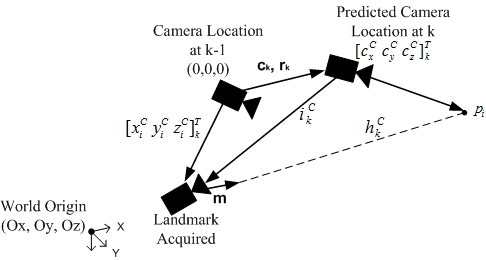
\includegraphics[width=10cm, keepaspectratio=true]{./Figures/measurement_model.jpg}
\caption{Measurement Model}
\label{fig:measurement_model}
\end{figure}

For a feature $p_{i}^{C}$, the vector $h^{R}$ pointing from the 
predicted camera location to the feature initialization position is 

\begin{equation}
h_{k}^{R}=\begin{bmatrix}
x_{i}^{C} \\
y_{i}^{C} \\
z_{i}^{C} \\
\end{bmatrix}_{k}-\begin{bmatrix}
c_{x}^{C} \\
c_{y}^{C} \\
c_{z}^{C} \\
\end{bmatrix}_{k}
\end{equation}

The normalized vector pointing from the predicted camera position to the 
feature at time k is then 

\begin{equation}
  h_{k}^{C}=Q^{-1}\left(r_{k}^{C}\right)\left(\rho _{k}h_{k}^{R}+m\left(\varphi_{ 
        k}^{C},\theta _{k}^{C}\right)\right)
\end{equation}

\noindent where $Q^{-1}(r_{k}^{C})$ is the inverse rotation matrix from the 
camera frame at time $k-1$ to camera frame at time $k$. From vector 
$h_{k}^{C}$, the feature location on image plane can be found by

\begin{equation}
h_{k}^{U}= \begin{bmatrix}
u_{k} \\
v_{k} \\
\end{bmatrix}=\begin{bmatrix}
\frac{f_{x}h_{y,k}^{C}}{h_{x,k}^{C}} \\
\frac{f_{y}h_{z,k}^{C}}{h_{x,k}^{C}} \\
\end{bmatrix}
\end{equation}

\noindent where $f_{x}$ and $f_{y}$ is the scaling factor of the projection, 
obtained through camera calibration.

\subsection{Composition Step}

Update step corrects the camera motion and feature location in camera 
frame k-1. To continue to the next cycle of tracking, all parameter must 
be transform to camera frame k. World reference point coordinate and 
orientation from k-1 to k is related by

\begin{equation}
\begin{bmatrix}
O_{x}^{C_{k}} \\
O_{y}^{C} \\
O_{z}^{C} \\
\end{bmatrix}_{k}=R^{-1}(r_{k}^{C_{k-1}})\left(
\begin{bmatrix}
O_{x}^{C_{k-1}} \\
O_{y}^{C_{k-1}} \\
O_{z}^{C_{k-1}} \\
\end{bmatrix}_{k}- \begin{bmatrix}
c_{x}^{C_{k-1}} \\
c_{y}^{C_{k-1}} \\
c_{z}^{C_{k-1}} \\
\end{bmatrix}_{k}\right)
\end{equation}

\begin{equation}
\begin{bmatrix}
W_{x}^{C_{k}} \\
W_{y}^{C_{k}} \\
W_{z}^{C_{k}} \\
\end{bmatrix}_{k-1}= \begin{bmatrix}
W_{x}^{C_{k-1}} \\
W_{y}^{C_{k-1}} \\
W_{z}^{C_{k-1}} \\
\end{bmatrix}_{k}-r^{C_{k-1}}
\end{equation}

Feature parameters in new camera frame are related to the previous frame 
by

\begin{equation}
\begin{bmatrix}
x_{i}^{C_{k}} \\
y_{i}^{C_{k}} \\
z_{i}^{C_{k}} \\
\end{bmatrix}_{k}=Q^{-1}(r^{C_{k-1}})\left(
\begin{bmatrix}
x_{i}^{C_{k-1}} \\
y_{i}^{C_{k-1}} \\
z_{i}^{C_{k-1}} \\
\end{bmatrix}_{k}- \begin{bmatrix}
c_{x}^{C_{k-1}} \\
c_{y}^{C_{k-1}} \\
c_{z}^{C_{k-1}} \\
\end{bmatrix}_{k}\right)
\end{equation}

\begin{equation}
\begin{bmatrix}
\rho_{i} \\
\varphi_{i}^{C_{k}} \\
\theta_{i}^{C_{k}} \\
\end{bmatrix}_{k}=
\begin{bmatrix}
\rho _{i, k} \\
m^{-1}(R^{-1}(r^{C_{k-1}})m(\varphi _{i, k}^{C_{k-1}}, \theta _{i, k}^{C_{k-1}}) \\
\end{bmatrix}
\end{equation}

\noindent where $m(\varphi_{i, k}^{C_{k-1}}, \theta_{i, k}^{C_{k-1}})$ is the 
unit vector pointing from the initialization point to the feature seen 
by the camera at step $k-1$

The covariance matrix is also affected by this transform. Therefore must 
be updated. The new covariance matrix is related to the old one by 

\begin{equation}
P_{k}^{C_{k}}=J_{C_{k-1}\to C_{k}}P_{k}^{C_{k-1}}J_{C_{k-1}\to C_{k}}^{T}
\end{equation}

The calculation of $J_{C_{k-1}\to C_{k}}$ is the same as the 
linearization of prediction matrix in section Method 2.

In order to apply the correction and update the camera reference frame
to the new camera position, an additional composition step is
necessary. The world reference frame parameters and features
parameters are updated by applying reference frame transformation from
the camera location at time $k-1$ to camera location at time k. The
EKF covariance matrix $P_{k}$ is also updated through

\begin{equation}
P_{k}=JP_{k}J^{T}
\end{equation}

\noindent where $J$ is the Jacobian of the composition equations. 
\section{Initialization}
\subsection{Initialize the State Vector}

State vectors are initialized at the first frame. The world origin 
coordinate and orientation, camera motions, and the feature reference 
points are all initialized to zeros, with variance equals to the 
smallest machine number. Thus, 

\begin{equation}
OX_{W}^{C}=\begin{bmatrix}0&0&0&0&0&0\end{bmatrix} 
\end{equation}

\begin{equation}
c^{C}=\begin{bmatrix}0&0&0\end{bmatrix}
\end{equation}

\begin{equation}
r^{C}=\begin{bmatrix}0&0&0\end{bmatrix}
\end{equation}

\begin{equation}
p_{i}^{C}=\begin{bmatrix}0&0&0&\rho _{i}&\varphi_{i}&\theta_{i}\end{bmatrix}
\end{equation}

The inverse distance $\rho $ of all features are initialized to 0.1 
because we are dealing with long distance object. The features 
elevation-azimuth pair $[\varphi _{i}^{C}, \theta _{i}^{C}]$ is 
extracted from features coordinates in image plane. First, a vector 
pointing from camera optical center to feature can be defined by

\begin{equation}
h^{C}=\begin{bmatrix}
h_{x}^{C}\\
h_{y}^{C}\\
h_{z}^{C}\\
\end{bmatrix}
 = \begin{bmatrix}
1 \\
u\cdot s_{x} \\
v\cdot s_{y} \\
\end{bmatrix}
\end{equation}

Where $[u v]$ is the feature coordinate in the image, and $
[s_{x}s_{y}] $is the scaling factor of the projection from the scene to 
image plane. The elevation-azimuth pair $[\varphi _{i}^{C}, \theta 
_{i}^{C}]$ can then be directly calculated from $h^{C}$

\begin{equation}
\varphi 
=arctan\left(\frac{h_{z}^{C}}{\sqrt{{h_{x}^{C}}^{2}+{h_{y}^{C}}^{2}}}\right)
\end{equation}

\begin{equation}
\theta =arctan\left(\frac{h_{y}^{C}}{h_{x}^{C}}\right)
\end{equation}


\subsection{Initialized the State Covariance Matrix}

Because the world origin is defined at the first frame, it enables 
initializing the filter with minimum variance, which helps reducing the 
lower bound of the filter error. The covariance matrix of the world 
coordinate and orientation, and the camera motion is 

\begin{equation}
P=I_{12\times 12}\cdot \epsilon 
\end{equation}

where $I$ is a $12\times12$ identity matrix, and $\epsilon $ is the 
lowest significant bit (LSB) of a machine.

The covariance of features is added one by one as there is 
correlation between them. For every new feature added, the new 
covariance matrix becomes

\begin{equation}
\label{eq:Pnew}
P_{new}=J\begin{bmatrix}
P_{old} & 0 \\
0 & R \\
\end{bmatrix}
J^{T}
\end{equation}

\noindent where $P_{old}$ is the covariance matrix of the existing state vector, 
and the initial $P_{old}$ is defined in . Matrix R is the covariance 
matrix of the variable in features initialization.

\begin{equation}
R=\begin{bmatrix}
\sigma _{x_{i}^{C}} & & & & & & \\
 & \sigma _{y_{i}^{C}} & & & 0 & & \\
 & & \sigma _{z_{i}^{C}} & & & & \\
 & & & \sigma _{\rho } & & & \\
 & 0 & & & \sigma _{image} & & \\
 & & & & & \sigma _{image} & \\
\end{bmatrix}
 = \begin{bmatrix}
\epsilon & & & & & & \\
 & \epsilon & & & 0 & & \\
 & & \epsilon & & & & \\
 & & & 0.1 & & & \\
 & 0 & & & 1 & & \\
 & & & & & 1 & \\
\end{bmatrix} 
\end{equation}

\noindent where$[\sigma_{x_{i}}^{C}, \sigma_{y_{i}}^{C}, \sigma
_{z_{i}}^{C}]$ is the uncertainty of the camera optical center
position, initialized to $\epsilon $.$\sigma _{image}$is the image
plane pixel variance, set to 1. $\sigma _{\rho }$is the uncertainty of
the inverse distance. Because the filter mainly deals with distance
feature, $ \sigma _{\rho }$ is initialized to 0.1 to cover any
distance from 50 meters to infinity.

$J$ in equation(\ref{eq:Pnew}) is the Jacobian matrix for 
the initialization equation. 

\begin{equation}
J=\begin{bmatrix}
 & & & & & &0\\
 & &I& & & &\vdots\\ 
 & & & & & &0\\
\frac{\partial p_{i}}{\partial OX_{W}^{C}} &
\frac{\partial p_{i}}{\partial c^{C}} & 
\frac{\partial p_{i}}{\partial r^{C}} & 
0 & \ldots & 0 & 
\frac{\partial p_{i}}{\partial g_{i}} 
\end{bmatrix}
\end{equation}

Whenever a new feature is added, it's initial position is always $
\begin{bmatrix}0&0&0\end{bmatrix}$ in the camera centric coordinate,
and the $\begin{bmatrix}\rho&\varphi&\theta\end{bmatrix}$ parameters
are not a function of $ OX_{W}^{C}$, $c^{C}$,or$r^{C}$, therefore

\begin{equation}
\frac{\partial p_{i}}{\partial OX_{W}^{C}}=0_{6\times 6}
\end{equation}

\begin{equation}
\frac{\partial p_{i}}{\partial c^{C}}=0_{6\times 3}\frac{\partial 
p_{i}}{\partial r^{C}}= 0_{6\times 3}
\end{equation}

$J$ can then be simplified as

\begin{equation}
J=\begin{bmatrix}
I & 0 & \\
0 & \frac{\partial p_{i}}{\partial g_{i}} & \\
\end{bmatrix} 
\end{equation}


\noindent where$g_{i}$ includes the variable in matrix $R$: $
g_{i}=[\begin{matrix}
x_{i}^{C} & y_{i}^{C} & z_{i}^{C} & \rho _{i} & u_{i} & v_{i}
\end{matrix}
]$. Then 

\begin{equation}
\frac{\partial p_{i}}{\partial g_{i}}=\begin{bmatrix}
I_{3\times 3} & & 0_{3\times 3} & \\
 & \frac{\partial \rho_{i}}{\partial \rho_{i}} & 
\frac{\partial \rho_{i}}{\partial u_{i}} & 
\frac{\partial \rho _{i}}{\partial v_{i}}\\
0_{3\times 3} & \frac{\partial \varphi_{i}^{C}}{\partial \rho_{i}} & 
\frac{\partial \varphi_{i}^{C}}{\partial u_{i}} & 
\frac{\partial \varphi_{i}^{C}}{\partial v_{i}} \\
 & \frac{\partial \theta_{i}^{C}}{\partial \rho_{i}} & 
\frac{\partial \theta_{i}^{C}}{\partial u_{i}} & 
\frac{\partial \theta_{i}^{C}}{\partial v_{i}} \\
\end{bmatrix} = \begin{bmatrix}
I_{3\times 3} & & 0_{3\times 3} & \\
 & 1 & 0 & 0 \\
0_{3\times 3} & 0 & \frac{\partial \varphi _{i}^{C}}{\partial u_{i}} 
& \frac{\partial \varphi_{i}^{C}}{\partial v_{i}} \\
 & 0 & \frac{\partial \theta_{i}^{C}}{\partial u_{i}} & 
\frac{\partial \theta_{i}^{C}}{\partial v_{i}} \\
\end{bmatrix}
\end{equation}

Based on the rule of derivation, 

$$\frac{\partial \varphi_{i}^{C}}{\partial u_{i}}=\frac{\partial 
\varphi_{i}^{C}}{\partial h^{C}}\frac{\partial h^{C}}{\partial u_{i}}$$


$$\frac{\partial \theta _{i}^{C}}{\partial u_{i}}=\frac{\partial \theta 
_{i}^{C}}{\partial h^{C}}\frac{\partial h^{C}}{\partial u_{i}}$$


$$\frac{\partial \varphi _{i}^{C}}{\partial v_{i}}=\frac{\partial 
\varphi _{i}^{C}}{\partial h^{C}}\frac{\partial h^{C}}{\partial v_{i}}$$

$$\frac{\partial \theta _{i}^{C}}{\partial v_{i}}=\frac{\partial \theta 
_{i}^{C}}{\partial h^{C}}\frac{\partial h^{C}}{\partial v_{i}}$$


\noindent and

\begin{equation}
\frac{\partial \varphi_{i}^{C}}{\partial h^{C}}= 
\begin{bmatrix}
\frac{\partial \varphi_{i}^{C}}{\partial h_{x}^{C}} & 
\frac{\partial \varphi_{i}^{C}}{\partial h_{y}^{C}} & 
\frac{\partial \varphi_{i}^{C}}{\partial h_{z}^{C}}
\end{bmatrix}=\begin{bmatrix}
\frac{-h_{x}^{C}\cdot h_{z}^{C}}{({h_{x}^{C}}^{2}+{h_{y}^{C}}^{2}+{h_{z}^{C}}^{2})\sqrt{{h_{x}^{C}}^{2}+{h_{y}^{C}}^{2}}} \\
\frac{-h_{y}^{W}\cdot h_{z}^{W}}{({h_{x}^{C}}^{2}+{h_{y}^{C}}^{2}+{h_{z}^{C}}^{2})\sqrt{{h_{x}^{C}}^{2}+{h_{y}^{C}}^{2}}} \\
\frac{\sqrt{{h_{x}^{C}}^{2}+{h_{y}^{C}}^{2}}}{({h_{x}^{C}}^{2}+{h_{y}^{C}}^{2}+{h_{z}^{C}}^{2})}
\end{bmatrix}^{T}
\end{equation}

\begin{equation}
\frac{\partial \theta_{i}^{C}}{\partial h^{C}}=\begin{bmatrix}
\frac{\partial \theta_{i}^{C}}{\partial h_{x}^{C}} & 
\frac{\partial \theta_{i}^{C}}{\partial h_{y}^{C}} & 
\frac{\partial \theta_{i}^{C}}{\partial h_{z}^{C}} \end{bmatrix}
=\begin{bmatrix}
-\frac{h_{y}^{C}}{{h_{x}^{C}}^{2}+{h_{y}^{C}}^{2}} & 
\frac{h_{x}^{C}}{{h_{x}^{C}}^{2}+{h_{y}^{C}}^{2}} & 0
\end{bmatrix}
\end{equation}

\begin{equation}
\frac{\partial h^{C}}{\partial u_{i}}=\begin{bmatrix}
\frac{\partial h_{x}^{C}}{\partial u_{i}} \\
\frac{\partial h_{y}^{C}}{\partial u_{i}} \\
\frac{\partial h_{z}^{C}}{\partial u_{i}} \\
\end{bmatrix}= \begin{bmatrix}
0 \\
s_{x}\\
0
\end{bmatrix}
\end{equation}

\begin{equation}
\frac{\partial h^{C}}{\partial v_{i}}=\begin{bmatrix}
\frac{\partial h_{x}^{C}}{\partial v_{i}}\\
\frac{\partial h_{y}^{C}}{\partial v_{i}}\\
\frac{\partial h_{z}^{C}}{\partial v_{i}}\\
\end{bmatrix}= \begin{bmatrix}
0 \\
0 \\
s_{y}\\
\end{bmatrix}
\end{equation}

\subsubsection{Linearization of Measurement Model}
The measurement model of the algorithm is not linear, and must be 
linearized by evaluating first derivative of the measurement equation at 
the predicted camera location. Since the measurement model is not a 
function of world origin coordinate and orientation, the Jacobian matrix 
of the measurement model is

\begin{multline}
\frac{\partial h_{k}^{U}(x)}{\partial x}=
\begin{bmatrix}
0_{2n\times 6} & \frac{\partial h_{k}^{U}(x)}{\partial c^{C}} &
\frac{\partial h_{k}^{U}(x)}{\partial r^{C}} &
\frac{\partial h_{k}^{U}(x)}{\partial p_{1}} & 
\ldots & \frac{\partial h_{k}^{U}(x)}{\partial p_{n}}
\end{bmatrix} = \\ \begin{bmatrix}
0_{2n\times 6} & 
\frac{\partial h_{k}^{U}}{\partial h_{k}^{C}} \cdot 
\frac{\partial h_{k}^{C}}{\partial c^{C}} & 
\frac{\partial h_{k}^{U}}{\partial h_{k}^{C}} \cdot 
\frac{\partial h_{k}^{C}}{\partial r^{C}} & 
\frac{\partial h_{k}^{U}}{\partial h_{k}^{C}} \cdot 
\frac{\partial h_{k}^{C}}{\partial p_{1}} & 
\ldots & 
\frac{\partial h_{k}^{U}}{\partial h_{k}^{C}} \cdot 
\frac{\partial h_{k}^{C}}{\partial p_{n}}
\end{bmatrix}
\end{multline}


Elements in the matrix above are given in - . The formula for 
calculating $Q^{-1}$in - can be found in 

\begin{equation}
\frac{\partial h_{k}^{U}}{\partial h_{k}^{C}}= \begin{bmatrix}
-\frac{s_{x}h_{y,k}^{C}}{{h_{x,k}^{C}}^{2}} & \frac{s_{x}}{h_{x,k}^{C}} & 0 \\
-\frac{s_{y}h_{z,k}^{C}}{{h_{x,k}^{C}}^{2}} & 0 & \frac{s_{y}}{h_{x,k}^{C}}
\end{bmatrix}
\end{equation}

\begin{equation}
\frac{\partial h^{C}}{\partial c^{C}}=-R^{-1}(r_{k}^{C})\rho _{k}
\end{equation}

\begin{equation}
\frac{\partial h(x)}{\partial r^{C}}=\begin{bmatrix} 
\frac{\partial h^{C}}{\partial r_{x}^{C}} & 
\frac{\partial h^{C}}{\partial r_{y}^{C}} & 
\frac{\partial h^{C}}{\partial r_{z}^{C}}\end{bmatrix}
\end{equation}


\begin{equation}
\frac{\partial h^{C}}{\partial r_{x}}=\begin{bmatrix}
0 \\
h_{x}^{C}(sin(r_{x})sin(r_{z})+cos(r_{x})cos(r_{z})sin(r_{y}))
+h_{y}^{C}(-cos(r_{z})sin(r_{x})+cos(r_{x})sin(r_{y})sin(r_{z})) 
+ h_{z}^{C}cos(r_{x})cos(r_{y}) \\
h_{x}^{C}(cos(r_{x})\sin(r_{z})-cos(r_{z})sin(r_{x})sin(r_{y}))+
h_{y}^{C}(-cos(r_{x})cos(r_{z})-sin(r_{x})sin(r_{y})sin(r_{z})) 
- h_{z}^{C}cos(r_{y})sin(r_{x}) \\
\end{bmatrix}
\end{equation}

\begin{equation}
\frac{\partial h^{C}}{\partial r_{y}}=\begin{bmatrix}
-h_{z}^{C}\cos(r_{y})-h_{x}^{C}\cos(r_{z})sin(r_{y})- 
h_{y}^{C}sin(r_{y})sin(r_{z}) \\
-h_{z}^{C}sin(r_{x})sin(r_{y})+
h_{x}^{C}cos(r_{y})cos(r_{z})sin(r_{x})+
h_{y}^{C}cos(r_{y})sin(r_{x})sin(r_{z}) \\
-h_{z}^{C}cos(r_{x})sin(r_{y})+
h_{x}^{C}cos(r_{x})cos(r_{y})cos(r_{z})+
h_{y}^{C}cos(r_{x})cos(r_{y})sin(r_{z}) \\
\end{bmatrix}
\end{equation}

\begin{equation}
\frac{\partial h^{C}}{\partial r_{z}}=\begin{bmatrix}
h_{y}^{C}cos(r_{y})cos(r_{z})-h_{x}^{C}cos(r_{y})sin(r_{z})\\
h_{x}^{C}(-cos(r_{x})\cos (r_{z})-sin(r_{x})\sin(r_{y})\sin (r_{z}))+ 
h_{y}^{C}(-cos(r_{x})sin(r_{z})+cos(r_{z})sin(r_{x})sin(r_{y}))\\
h_{x}^{C}(cos(r_{z})sin(r_{x})-cos(r_{x})sin(r_{y})sin(r_{z}))+
h_{y}^{C}(sin(r_{x})sin(r_{z})+cos(r_{x})cos(r_{z})sin(r_{y}))\\
\end{bmatrix}
\end{equation}

\begin{equation}
\frac{\partial h^{C}}{\partial p_{i}}=\begin{bmatrix}
\frac{\partial h^{C}}{\partial x_{i}^{C}} & 
\frac{\partial h^{C}}{\partial y_{i}^{C}} & 
\frac{\partial h^{C}}{\partial z_{i}^{C}} & 
\frac{\partial h^{C}}{\partial \rho _{i}} &
\frac{\partial h^{C}}{\partial \theta _{i}} &
\frac{\partial h^{C}}{\partial \varphi _{i}}
\end{bmatrix}
\end{equation}

Equation above is a 3x6 matrix

\begin{equation}
\begin{bmatrix}
\frac{\partial h^{C}}{\partial x_{i}^{C}} & 
\frac{\partial h^{C}}{\partial y_{i}^{C}} & 
\frac{\partial h^{C}}{\partial z_{i}^{C}}
\end{bmatrix}
 =Q^{-1}(r_{k}^{C})\rho _{k}
\end{equation}


\begin{equation}
\frac{\partial h^{C}}{\partial \rho _{i}}=-Q^{-1}(r_{k}^{C})\cdot c_{k}
\end{equation}


\begin{equation}
\frac{\partial h^{C}}{\partial \theta _{i}}=
Q^{-1}(r_{k}^{C}) \begin{bmatrix}
-cos(\varphi _{i})\sin(\theta _{i}) \\
\cos (\varphi _{i})cos(\theta _{i}) \\
0 \end{bmatrix}
\end{equation}

\begin{equation}
\frac{\partial h^{C}}{\partial \varphi _{i}}= 
Q^{-1}(r_{k}^{C}) \begin{bmatrix}
-cos(\varphi _{i})sin(\theta _{i}) \\
-sin(\varphi _{i})sin(\theta _{i}) \\
cos(\varphi _{i})
\end{bmatrix}
\end{equation}

\subsubsection{Jacobian Matrix of Composition Equations}

\begin{equation}
J_{C_{k-1}\to C_{k}}=\frac{\partial x_{k}}{\partial x_{k-1}}=\begin{bmatrix}
\frac{\partial x_{k}}{\partial OX_{W, k-1}^{C}} &
\frac{\partial x_{k}}{\partial c_{k-1}} & 
\frac{\partial x_{k}}{\partial r_{k-1}} & 
\frac{\partial x_{k}}{\partial p_{1, k-1}^{C}} &
\frac{\partial x_{k}}{\partial p_{2, k-1}^{C}} &
\cdots 
\end{bmatrix}
\end{equation}

$\frac{\partial x_{k}}{\partial OX_{W, k-1}^{C}}$is given by:

\begin{equation}
\frac{\partial x_{k}}{\partial OX_{W, k-1}^{C}}=\begin{bmatrix}
\frac{\partial O_{W,k}^{C}}{\partial O_{W,k-1}^{C}} & 
\frac{\partial O_{W,k}^{C}}{\partial W_{W,k-1}^{C}} \\
\frac{\partial W_{W,k}^{C}}{\partial O_{W,k-1}^{C}} & 
\frac{\partial W_{W,k}^{C}}{\partial W_{W,k-1}^{C}} \\
\frac{\partial c_{k}}{\partial O_{W,k-1}^{C}} &
\frac{\partial c_{k}}{\partial W_{W,k-1}^{C}} \\
\frac{\partial r_{k}}{\partial O_{W,k-1}^{C}} &
\frac{\partial r_{k}}{\partial W_{W,k-1}^{C}} \\
\frac{\partial p_{i}^{C}}{\partial O_{W,k-1}^{C}} & 
\frac{\partial p_{i}^{C}}{\partial W_{W,k-1}^{C}} \\
\end{bmatrix}= \begin{bmatrix}
Q^{-1}(r^{C}) & 0 \\
0 & I_{3\times 3} \\
0 & 0 \\
0 & 0 \\
0 & 0 
\end{bmatrix}
\end{equation}


Derivatives of $x_{k}$with respect to $c$ and $p$are given in - 


\begin{equation}
\begin{bmatrix}
\frac{\partial O_{W,k}^{C}}{\partial c_{k-1}} & 
\frac{\partial O_{W,k}^{C}}{\partial r_{k-1}} \\
\frac{\partial W_{W,k}^{C}}{\partial c_{k-1}} &
\frac{\partial W_{W,k}^{C}}{\partial r_{k-1}} \\
\frac{\partial c_{k}}{\partial c_{k-1}} & 
\frac{\partial c_{k}}{\partial r_{k-1}} \\
\frac{\partial r_{k}}{\partial c_{k-1}} & 
\frac{\partial r_{k}}{\partial r_{k-1}} \\
\frac{\partial p(0:2)_{i}^{C}}{\partial c_{k-1}} & 
\frac{\partial p(0:2)_{i}^{C}}{\partial r_{k-1}} \\
\frac{\partial p(3:5)_{i}^{C}}{\partial c_{k-1}} & 
\frac{\partial p(3:5)_{i}^{C}}{\partial r_{k-1}} \\
\end{bmatrix}= \begin{bmatrix}
-Q^{-1}(r_{k}^{C_{k-1}}) & 
\frac{\partial Q^{-1}(r_{k}^{C_{k-1}})}{\partial r_{k-1}} \\
0_{3\times 3} & -I_{3\times 3} \\
I_{3\times 3} & 0_{3\times 3} \\
0_{3\times 3} & I_{3\times 3} \\
-Q^{-1}(r_{k}^{C_{k-1}}) & 
\frac{\partial Q^{-1}(r_{k}^{C_{k-1}})}{\partial r_{k-1}} \\
0_{3\times 3} & pr 
\end{bmatrix}
\end{equation}

\noindent where

\begin{equation}
pr=\begin{bmatrix}
1 & 0 & 0 & \\
&\frac{\partial \varphi _{i, k}^{C}}{\partial r_{k-1}} & \\
&\frac{\partial \theta _{i, k}^{C}}{\partial r_{k-1}} & \\
\end{bmatrix}= \begin{bmatrix}
1 & 0 & 0 \\
&\frac{\partial m^{-1}(Q^{-1}(r_{k}^{C_{k-1}})m(\varphi _{i, 
k}^{C_{k-1}}, \theta _{i, k}^{C_{k-1}}))}{\partial r_{k-1}} & \\
\end{bmatrix}
\end{equation}

Let $M=Q^{-1}(r_{k}^{C_{k-1}})m(\varphi_{i, k}^{C_{k-1}}, \theta _{i, 
k}^{C_{k-1}})$, and $m^{-1}=m^{-1}(M)$, then

\begin{equation}
\frac{\partial m^{-1}}{\partial r_{k}^{C_{k-1}}}=
\frac{\partial m^{-1}}{\partial M}\cdot 
\frac{\partial M}{\partial r_{k}^{C_{k-1}}}
\end{equation}

\noindent where

\begin{equation}
\frac{\partial M}{\partial r_{k}^{C_{k-1}}}= 
\frac{\partial Q^{-1}(r_{k}^{C_{k-1}})}{\partial r_{k-1}}
\cdot m(\varphi_{i, k}^{C_{k-1}}, \theta_{i, k}^{C_{k-1}})
\end{equation}


\noindent as $m^{-1}$ isthe function that calculate
$\begin{bmatrix}\varphi & \theta \end{bmatrix}$ from a 
vector,$\frac{\partial m^{-1}}{\partial M}$ is the same as and .

Derivatives of $x_{k}$ with respect to feature parameters $p_{i}^{C}
$are given in

\begin{equation}
\frac{\partial x_{k}^{C_{k}}}{\partial p_{i,k}^{C_{k-1 }}}=
\begin{bmatrix}
\frac{\partial O_{W,k}^{C_{k}}}{\partial p_{i,k}^{C_{k-1 }}} \\
\frac{\partial W_{W,k}^{C_{k}}}{\partial p_{i,k}^{C_{k-1 }}} \\
\frac{\partial c_{k}^{C_{k}}}{\partial p_{i,k}^{C_{k-1 }}} \\
\frac{\partial r_{k}^{C_{k}}}{\partial p_{i,k}^{C_{k-1 }}} \\
\frac{\partial p_{i, k}^{C}}{\partial p_{i,k}^{C_{k-1 }}} \\
\end{bmatrix} = \begin{bmatrix}
0 \\
0 \\
0 \\
0 \\
\frac{\partial p_{i,k}^{C_{k }}}{\partial p_{i,k}^{C_{k-1 }}} \\
\end{bmatrix}
\end{equation}


\begin{equation}
\frac{\partial p_{i,k}^{C_{k }}}{\partial p_{i,k}^{C_{k-1 }}}=
\begin{bmatrix}
\frac{\partial x_{i,k}^{C_{k}}}{\partial p_{i,k}^{C_{k-1 }}} \\
\frac{\partial y_{i,k}^{C}}{\partial p_{i,k}^{C_{k-1 }}} \\
\frac{\partial z_{i,k}^{C}}{\partial p_{i,k}^{C_{k-1 }}} \\
\frac{\partial \rho _{i,k}^{C}}{\partial p_{i,k}^{C_{k-1 }}} \\
\frac{\partial \varphi _{i, k}^{C}}{\partial p_{i,k}^{C_{k-1 }}} \\
\frac{\partial \theta _{i, k}^{C}}{\partial p_{i,k}^{C_{k-1 }}} \\
\end{bmatrix}=\begin{bmatrix}
Q^{-1}(r_{k}^{C_{k-1}}) & 0_{3\times 3} \\
0_{3\times 3} & 
\frac{\partial p(3:5)_{i,k}^{C_{k}}}{\partial p(3:5)_{i,k}^{C_{k-1}}} \\
\end{bmatrix}
\end{equation}


\begin{equation}
\frac{\partial p(3:5)_{i,k}^{C_{k}}}{\partial p(3:5)_{i,k}^{C_{k-1}}}=
 \begin{bmatrix}
1 & 0 & 0 \\
0 & 
\frac{\partial \varphi_{i, k}^{C_{k}}}
{\partial \varphi_{i,k}^{C_{k-1}}} & 
\frac{\partial \varphi _{i, k}^{C_{k}}}
{\partial \theta _{i, k}^{C_{k-1}}} \\
0 & 
\frac{\partial \theta _{i, k}^{C_{k}}}
{\partial \varphi _{i, k}^{C_{k-1}}} & 
\frac{\partial \theta _{i, k}^{C_{k}}}
{\partial \theta _{i, k}^{C_{k-1}}} \\
\end{bmatrix}=\begin{bmatrix}
1 & 0 & 0 \\
0 & 
\frac{\partial \varphi _{i, k}^{C_{k}}}{\partial M}
\frac{\partial M}{\partial \varphi _{i, k}^{C_{k-1}}} & 
\frac{\partial \varphi _{i,k}^{C_{k}}}
{\partial M}\frac{\partial M}{\partial \theta _{i,k}^{C_{k-1}}}\\
0 & 
\frac{\partial \theta _{i, k}^{C_{k}}}{\partial M}
\frac{\partial M}{\partial \varphi _{i, k}^{C_{k-1}}} & 
\frac{\partial \theta _{i,k}^{C_{k}}}{\partial M}
\frac{\partial M}{\partial \theta _{i, k}^{C_{k-1}}} \\
\end{bmatrix}
\end{equation}

\noindent in which $\frac{\partial \varphi _{i, k}^{C_{k}}}{\partial
  M}$ is the same as equation \ref{}. $\frac{\partial \theta _{i,
    k}^{C_{k}}}{\partial M}$ is the same as equation \ref{} . $\frac{\partial
  M}{\partial \varphi _{i,k}^{C_{k-1}}}$ and $ \frac{\partial
  M}{\partial \theta _{i, k}^{C_{k-1}}}$ is given below.

\begin{equation}
\frac{\partial M}{\partial \varphi_{i,k}^{C_{k-1}}}=
R^{-1}(r^{C})\begin{bmatrix}
-\cos(\theta_{i, k}^{C_{k-1}})\sin(\varphi_{i,k}^{C_{k-1}}) \\
-\sin(\varphi_{i,k}^{C_{k-1}})\sin(\theta_{i, k}^{C_{k-1}}) \\
\cos (\varphi_{i,k}^{C_{k-1}})
\end{bmatrix}
\end{equation}

\begin{equation}
\frac{\partial M}{\partial \theta _{i,k}^{C_{k-1}}}=
R^{-1}(r^{C}) \begin{bmatrix}
-\cos(\varphi_{i,k}^{C_{k-1}})\sin(\theta_{i, k}^{C_{k-1}})\\
\cos(\varphi_{i,k}^{C_{k-1}})\cos(\theta_{i, k}^{C_{k-1}})\\
0\\
\end{bmatrix}
\end{equation}

\subsubsection{Adding and Deleting Features}\label{section:_Toc332876136}
Features that move out of the camera's FOI are removed from the filter. 
The removal is done by directly deleting the parameters from the state 
vector, and the related rows and columns from the state covariance 
matrix. The parameters of the deleted features are still recorded into 
the database, and remained unchanged for all iteration after the removal 
unless a GPS bundle correction occurs. 

To maintain sufficient amount of features to generate map, new features 
are acquired and added to the filter if a feature deletion procedure 
occurred, or number of tracked feature is lower than a threshold. The 
feature addition procedure occurs after the composition step of an 
iteration, and follows the same procedure as described in section . 

\subsubsection{Bundle Correction with GPS (not yet implemented)}
Apply overall correction on the map at a sparser time interval using the 
GPS positions. 

\subsubsection{Processing for Comparison to Ground Truth Data}
The accuracy of the result was analyzed by comparing to the digital 
elevation models (DEM) .To make the comparison, the features coordinate 
and the DEM data must be brought to the same coordinate system. For ease 
of viewing, the world coordinate is used. The features' positions can be 
converted to Euclidean representation in world frame by: 

\begin{equation} 
\begin{bmatrix}
X_{i}^{W} \\
Y_{i}^{W} \\
Z_{i}^{W} \\
\end{bmatrix}
=Q^{-1}(O_{XYZ}^{c}, W_{XYZ}^{c})(\begin{bmatrix}
x_{i}^{C} \\
y_{i}^{C} \\
z_{i}^{C} \\
\end{bmatrix}
+\frac{1}{\rho _{i}}m(\varphi _{i}^{C}, \theta _{i}^{C}))
\end{equation}

The DEM is converted into the world frame using the UAV's initial GPS
location $\begin{bmatrix} Latitude_{init} & Longitude_{init} &
  Height_{init} \end{bmatrix}$ and orientation$\begin{bmatrix}
  Roll_{init} & Pitch_{init } & Azimuth_{init} \end{bmatrix}$. First,
the UAV's GPS latitude and longitude is converted into UTM
representation $\begin{bmatrix} Northing_{init} & Easting_{init} &
  Height_{init} \end{bmatrix}$. Then, a transformation matrix can be
defined as followed:


\begin{equation}
Q_{Roll}^{-1}=\begin{bmatrix}
1 & 0 & 0 & 0 \\
0 & \cos (Roll_{init}) & \sin (Roll_{init}) & 0 \\
0 & -sin(Roll_{init}) & \cos (Roll_{init}) & 0 \\
0 & 0 & 0 & 1 \\
\end{bmatrix}
\end{equation}


\begin{equation}
Q_{Pitch}^{-1}=\begin{bmatrix}
\cos (Pitch_{init}+\pi ) & 0 & -\sin (Pitcch_{init}+\pi ) & 0 \\
0 & 1 & 0 & 0 \\
\sin (Pitch_{init}+\pi ) & 0 & \cos (Pitch_{init}+\pi ) & 0 \\
0 & 0 & 0 & 1 \\
\end{bmatrix}
\end{equation}

\begin{equation}
Q_{Azimuth}^{-1}=\begin{bmatrix}
\cos (Azimuth_{init}+\frac{\pi }{2}) & \sin (Azimuth_{init}+\frac{\pi 
}{2}) & 0 & 0\\
-sin(Azimuth_{init}+\frac{\pi }{2}) & \cos (Azimuth_{init}+\frac{\pi 
}{2}) & 0 & 0 \\
0 & 0 & 1 & 0 \\
0 & 0 & 0 & 1 \\
\end{bmatrix}
\end{equation}


\begin{equation}
Q_{T}^{-1}=\begin{bmatrix}
1 & 0 & 0 & -Northing_{init} \\
0 & 1 & 0 & -Easting_{init} \\
0 & 0 & 1 & -Height_{init} \\
0 & 0 & 0 & 1 \\
\end{bmatrix}
\end{equation}

\begin{equation}
Q^{-1}=Q_{T}^{-1}\cdot Q_{Roll}^{-1}\cdot Q_{Pitch}^{-1}\cdot Q_{Azimuth}^{-1}
\end{equation}

At last, the DEM in world coordinate is given by

$DEM_{World}=Q^{-1}\cdot DEM_{UTM}$



%%% Local Variables:
%%% mode: latex
%%% TeX-master: "thesis"
%%% End:
